\documentclass{sig-alternate-15}
\usepackage{subscript}
\usepackage{tikz}
\usepackage{hyperref}
\usepackage{graphicx}
\usepackage{amsmath}
\usepackage{cases}
\usepackage[lined,boxed,longend,ruled]{algorithm2e}
\usepackage[overload]{empheq}
\newcommand\mycommfont[1]{\footnotesize\ttfamily\textcolor{blue}{#1}}
\SetCommentSty{mycommfont}
\SetKwProg{Fn}{def}{\string:}{end}
\SetKwFunction{CompGrid}{Compute\_Grid}
\SetKwFunction{CompTop}{Compute\_Topics}
\SetKwFunction{CompComArea}{Compute\_intersection}
\SetKwFunction{CompDiffArea}{Compute\_difference}
\SetKwFunction{CrDT}{Create\_DataFrames}
\SetStartEndCondition{ }{}{}
\SetKw{KwTo}{in}\SetKwFor{For}{for}{\string:}{end for}
\newcommand{\forcond}{$df$ \KwTo{$dist\_clust\_pages$}}
\newcommand{\forRecDiff}{$map$ \KwTo{$commonAreas$}}
\newcommand{\forRecCom}{$map$ \KwTo{$computedMaps$}}
\AlgoDontDisplayBlockMarkers\SetAlgoNoEnd\SetAlgoNoLine
\graphicspath{ {./imgs/} }

\begin{document}

\title{DBB: Density Based [k-means] Bootstrap}

\numberofauthors{2}
\author{
    \alignauthor{}
    Gianluca Bortoli\\
           \affaddr{DISI\,-\,University of Trento}\\
           \affaddr{Student id: 179816}\\
           \email{gianluca.bortoli@studenti.unitn.it}
    \alignauthor{}
    Martin Brugnara\\
           \affaddr{DISI\,-\,University of Trento}\\
           \affaddr{Student id: 182904}\\
           \email{mb@disi.unitn.eu}
    }
\maketitle


\begin{abstract}
Abstract here
\end{abstract}


\printccsdesc{}
\keywords{Big data, Data mining, Clustering, Streaming, Parallel computation}


\section{Introduction}
The clustering problem consists in grouping together data items that are ``similar'' to each other such that the inter-group similarity is high, while the intra-group one is low.

This challenge has received a lot of attention over the years.
According to Jane and K.~\cite{jain2010data}, the first specific study appeared in 1954~\cite{10.2307/2342679} and by now thousends of solutions have been proposed.

Data clustering has been used in many different disciplines, such as
data mining~\cite{fayyad1996advances}, statistics~\cite{tijms1994stochastic,banfield1993model} and machine learning.
The most common usages aim to gain insight to data (underlying structure) and for summarizing it through cluster prototypes (compression).

The concept of similarity varies a lot in the different contexts it can be applied.
For example the Euclidean distance~(L2) can be used when dealing with continuous values or the Jaccard similarity index, which computes similarity for generic sets of elements.
Nonetheless, the underlying algorithm is agnostic with respect to the similarity measure that is applied to compute a distance between the elements in the data.
Clustering can be also viewed as identifying the dense regions of the probability density of the data source~\cite{bradley1998scaling}.

The literature suggests two different approaches: \emph{partitional} and \emph{hierarchical}.

The first strategy needs some parameters to be set and known in advance.
For example the \emph{k-means}, which is one of the most popular and adopted algorithm,
requires the number of cluster to be found~(\emph{K}).

The latter can be implemented both in a top down (divisive) or a bottom up (agglomerative) manner.
Initially, the divisive algorithm treats all data as a single big cluster and later splits it until every object is separated~\cite{kaufman2009finding}.
On the contrary, the agglomerative starts considering each ``element'' as a \emph{singleton} (a cluster composed of one element).
Next, the most similar clusters are collapsed together until only one big cluster remains.
Implicitly the merging order defines a clear hierarchy among the intermediate representations (dendrogram).

Clearly, both the above mentioned approaches to the clustering problem have their disadvantages.
The partitional methods require prior knowledge on the data distribution, while the hierarchical ones imply the user interaction to decide the dendrogram's cut height.
For a complete list of the various clustering tequnique flavours refer to Jan \emph{et al.} review~\cite{jain2010data}.
However, a solution that does not suffer from those is still an open challenge.

In this work we propose a completely autonomous system which merges the two strategies to overcome their weaknesses, meaning that it satisfies the following \emph{Data Mining Desiderata}:
\begin{enumerate}
    \item \textbf{streaming}: require one scan of the database, since reading from secondary memory is still the most costly I/O operation.
    Moreover the analysis can be stopped and restarted without having to re-process the whole data (``stop and resume'' support).
    This property adds the capability to incorporate additional data with existing model efficiently (incremental computation).
    \item \textbf{on-line ``anytime'' behaviour}: a ``best'' answer is always available at any time during the computation phase.
    \item \textbf{limited memory}: the tool must work within the bounds of a given amount of main memory (RAM).
    % TODO: vorrei che fosse anche parallelizzabile
\end{enumerate}


\section{Related work}
\label{related}
The most popular and simplest partitional algorithm is \textbf{k-means}~\cite{macqueen1967some}.
Like every other solution belonging to this class, it requires the objective number of clusters~($k$) to be known a-priori.
Unfortunately, there exists no mathematical formula to compute such parameter in advance,
requiring the test to be run multiple times with different values in order to find the best solution according to some criterion (\emph{e.g.} the Schwarz Criterion~\cite{schwarz1978estimating}).
This algorithm is based on the notion of distance and it is usually employs the Euclidean one.
The resulting division into clusters can be also seen as a lossy compression of the points towards the centroids identifying the clusters.
The main idea behind the k-means consists in minimizing an objective function.
Usually the Mean Squared Error~(MSE) is chosen, where the error is defined as the distance between each point and the centroid of the cluster it is assigned to.
This process is iterative; initially $k$ points are identified to be the centroids,
then all the points are assigned to the nearest centroid (locally minimazing the MSE)
and finally the centroids are recomputed as the barycenter of the clusters.
The procedure continues until the convergence of the centroids' locations.
A noteworthy aspect is that the bootstrap phase, namely the initial centroids identification, highly influences the outcome.

Different centroids usually lead to different results, since the algorithm is designed to find a local optimum.
Several options for the bootstrap have been proposed like the one from Bradley and Fayyad~\cite{bradley1998refining}.
They suggest to run the k-means algorithm $M$ times using any initial centroid selection strategy
on $M$ different subsets of the initial data.
After that, an optimal grouping of the $M \times k$ centroids identified in the previous runs has to be found.
Given the small set size, a brute force approach is a reasonable option.
Finally the ``real'' k-means will use those centroids as the initial ones.

Using a distance as a similarity measure implies that the clusters will have a spherical shape.
It follows that the algorithm performs best when the input data have features values that are normally distributed.

Despite these disadvantages, many variants and optimizations have been proposed both by the industrial and academic communities~\cite{kanungo2002efficient,likas2003global,elkan2003using}.\\


Another important clustering algorithm is the ``Density-based spatial clustering of applications with noise'', more commonly known as \textbf{DBSCAN}~\cite{ester1996density}.
As the name suggests, it is a density-based approach to the clustering problem,
meaning that it groups together points with many others in the neighborhood
and penalizes the ones in low density areas (outliers).
The original version of DBSCAN relies on two user-provided parameters, namely \emph{minPts} and $\epsilon$.
The \emph{minPts} variable represents the minimum number of points that must lie in a circle of radius $\epsilon$~(neighborhood).

This algorithm exploits the \emph{density-reachability} to define three classes of points:
\begin{itemize}
    \item \emph{core}: set of points that have at least \emph{minPts} neighbors.
    \item \emph{reachable}:
        set of points that are in the neighborhood of a \emph{core} point,
        but are not \emph{core} points themselves.
    \item \emph{outlier}:
        set of points that have less than \emph{minPts} points in their neighborhood.
\end{itemize}

As happens with the k-means, DBSCAN has the disadvantage of requiring its parameters \emph{minPts} and $\epsilon$ to be known in advance.
One possible solution is to let a domain expert deal with it, providing sensible parameters based on his prior and deep knowledge of the dataset.
Moreover, DBSCAN lacks in flexibility since it uses a single ``is dense'' threshold derived from the two input parameters.

Some techniques for estimating such parameters have been proposed in the literature, resulting in an extended version of the algorithm known as EDBSCAN~\cite{elbatta2013dynamic, ram2009enhanced}.
It improves the handling of local density variation that exists within the clusters and dynamically chooses the best \emph{minPts} and $\epsilon$ values for the current run.
For good clustering results, such significant density variation might be allowed within a cluster if the objective is not a large number of smaller unimportant clusters.
Furthermore, it tries to detect the clusters with different shapes and sizes that differ in local density.

As opposed to k-means, DBSCAN is able to find arbitrarly-shaped clusters, since it does not employ a distance to measure similarity.
Moreover, the notion of density-reachability is not symmetric.
Hence, this is the key property that allows to find clusters with any shape rather than only ones normally distributed.\\


There exist also mixed approaches that try to combines the advantages of both the partitional and the hierarchical models to overcome the respective weaknesses.

A noteworthy application is the \textbf{BFR}~\cite{bradley1998scaling} algorithm proposed by Bradley, Fayyad and Reina.
It adresses the problem of clustering very large databases that do not fit in main memory, where scanning data at each iteration step is extremely costly. This can be generalized to scenarios where random reading operations are costly or not possible (\emph{e.g.} streaming data, hard disk, non-materialized views).
The main idea behind BFR is to use sufficent statistics~\cite{fisher1922mathematical} to represent groups of points.

In more detail, first the algorithm has to be initialized with $k$ points, which are designated as the intial centroids.
After that, it fetches data filling the preallocated RAM buffer, and then
it updates the internal model (\emph{i.e.} it runs a classic k-means on the buffered data) and classifies the
singleton items into the following sets in order to perform \emph{data compression}:
\begin{enumerate}
    \item \emph{discard}: points that can be discarded after updating the sufficent statistics of the cluster they are assigned to.
    \item \emph{compression}: non discarded points that do not belong to any of the $k$ clusters,
        but can be summarized and reppresend by other sufficient statistics.
    \item \emph{retained}: points that do not belong to any of the previous classes.
        They are kept as is in the buffer.
\end{enumerate}
This data compression procedure is used to eliminate data points that are not useful anymore from main memory, thus allowing
the buffer to continuously accomodate new data.
To achive this, \emph{primary} data compression removes data points that are unlikely to change cluster membership in future
iterations thresholding the Mahalanobis radius~\cite{duda60} around a candidate centroid and summarizing all the items within that area (discard set).
Moreover, \emph{secondary} data compression aims at finding sub-clusters of points that are very close to each other that
were not compressed during the primary step (compression set).

Unfortunately, the BFR algorithm suffers from the cluster's shape issue as the k-means. Therefore, this approach is able to deal only with
data that follows a Gaussian distribution.

\section{Problem definition}
Clustering is the task of gathering toghether items in a way that elements belonging
to the same group (the \emph{cluster}) are more similar to each other other than the ones
assigned to the other clusters.\\
More formally, the input is composed of:
\begin{itemize}
    \item $X = \{x_0, \dots ,x_n\}$, the initial set of elements.
    \item $d: X \times X \to \mathbb{R}$, a \emph{metric} measuring the similarity.
\end{itemize}
The final goal is to find the cluster configuration
\begin{equation*}
    C = \left\{ C_0, \dots , C_m \right\}
\end{equation*}
partitioning $X$
into $m$ clusters optimizing the following multi-objective function:\\

$f\left(2^X\right) =$
\begin{math}
    \left\{
        \begin{array}{l}
            \text{minimize the intra-cluster distance}
            \\
            \text{maximize the inter-cluster distance}
        \end{array}
    \right.
\end{math}

\section{Solution}
This work consists in solving the two main problems of ``k-means''-like
algorithms described in Section \ref{related} and \ref{problem_definition}:
choosing the $k$ parameter and placing the $k$ initial centroids.
The only assumption is that the dataset is generated from one or more gaussian
disitributions.


\subsection{The choice of $k$}
The most common scenario does not involve a domain expert. As a matter of fact,
no prior knowledge can be used to guess a proper and reasonable value for $k$.\\
The main idea behind the solution proposed in this work is that of exploiting global
and local density analysis to get an initial estimate of the number of clusters
in the data.

More formally, a \emph{peak detection} procedure is used to retrieve
all the peaks (i.e. local maxima) in the density function for each feature\footnote{If
the item considered is a point in an n-dimensional euclidean space, this is equivalent to
finding all the local maxima in the density functions for each axis.} of the items in
the dataset. In this way, a \emph{peak} is a data sample that is larger than
its two neighbour samples.
This results in a list of peaks for each feature space and finally a n-dimensional grid
matching every possible peak among all the features available is created
(see Algorithm \ref{alg:grid_creation}).
\begin{algorithm}[h]
 \KwIn{xs, points'x values}
 \KwIn{ys, points'y values}
 \KwResult{array, initial centroids}

 hx = computeMarginalDensity (xs)\;
 hy = computeMarginalDensity (ys)\;

 px = detectPeaks (hx)\;
 py = detectPeaks (hy)\;

 centroids = []\;
 \For{i $\in$ px}{
    \For{j $\in$ py}{
        centroids += (hx.x[i], hy.x[j])\;
    }
 }
% return [(hx[x], hy[y]) for x in px for y in py]
 \KwRet{centroids}
 \caption{Initial centroids identification}\label{alg:grid_creation}
\end{algorithm}


As Figure~\ref{grid} shows, the black diamonds on the top and on
the left sub-figures are the peaks found on the density distribution function among all
the points in the dataset, while the orange points in the central sub-figure represent the
grid of all the potential centroids.
In this way, the worst-case scenario is taken into account, allowing this approach not
to miss any potential centroid in the whole dataset\footnote{This approach produces an
over-estimation of the real number of centroids, introducing possible false-negatives.}.

\begin{figure*}
  \center{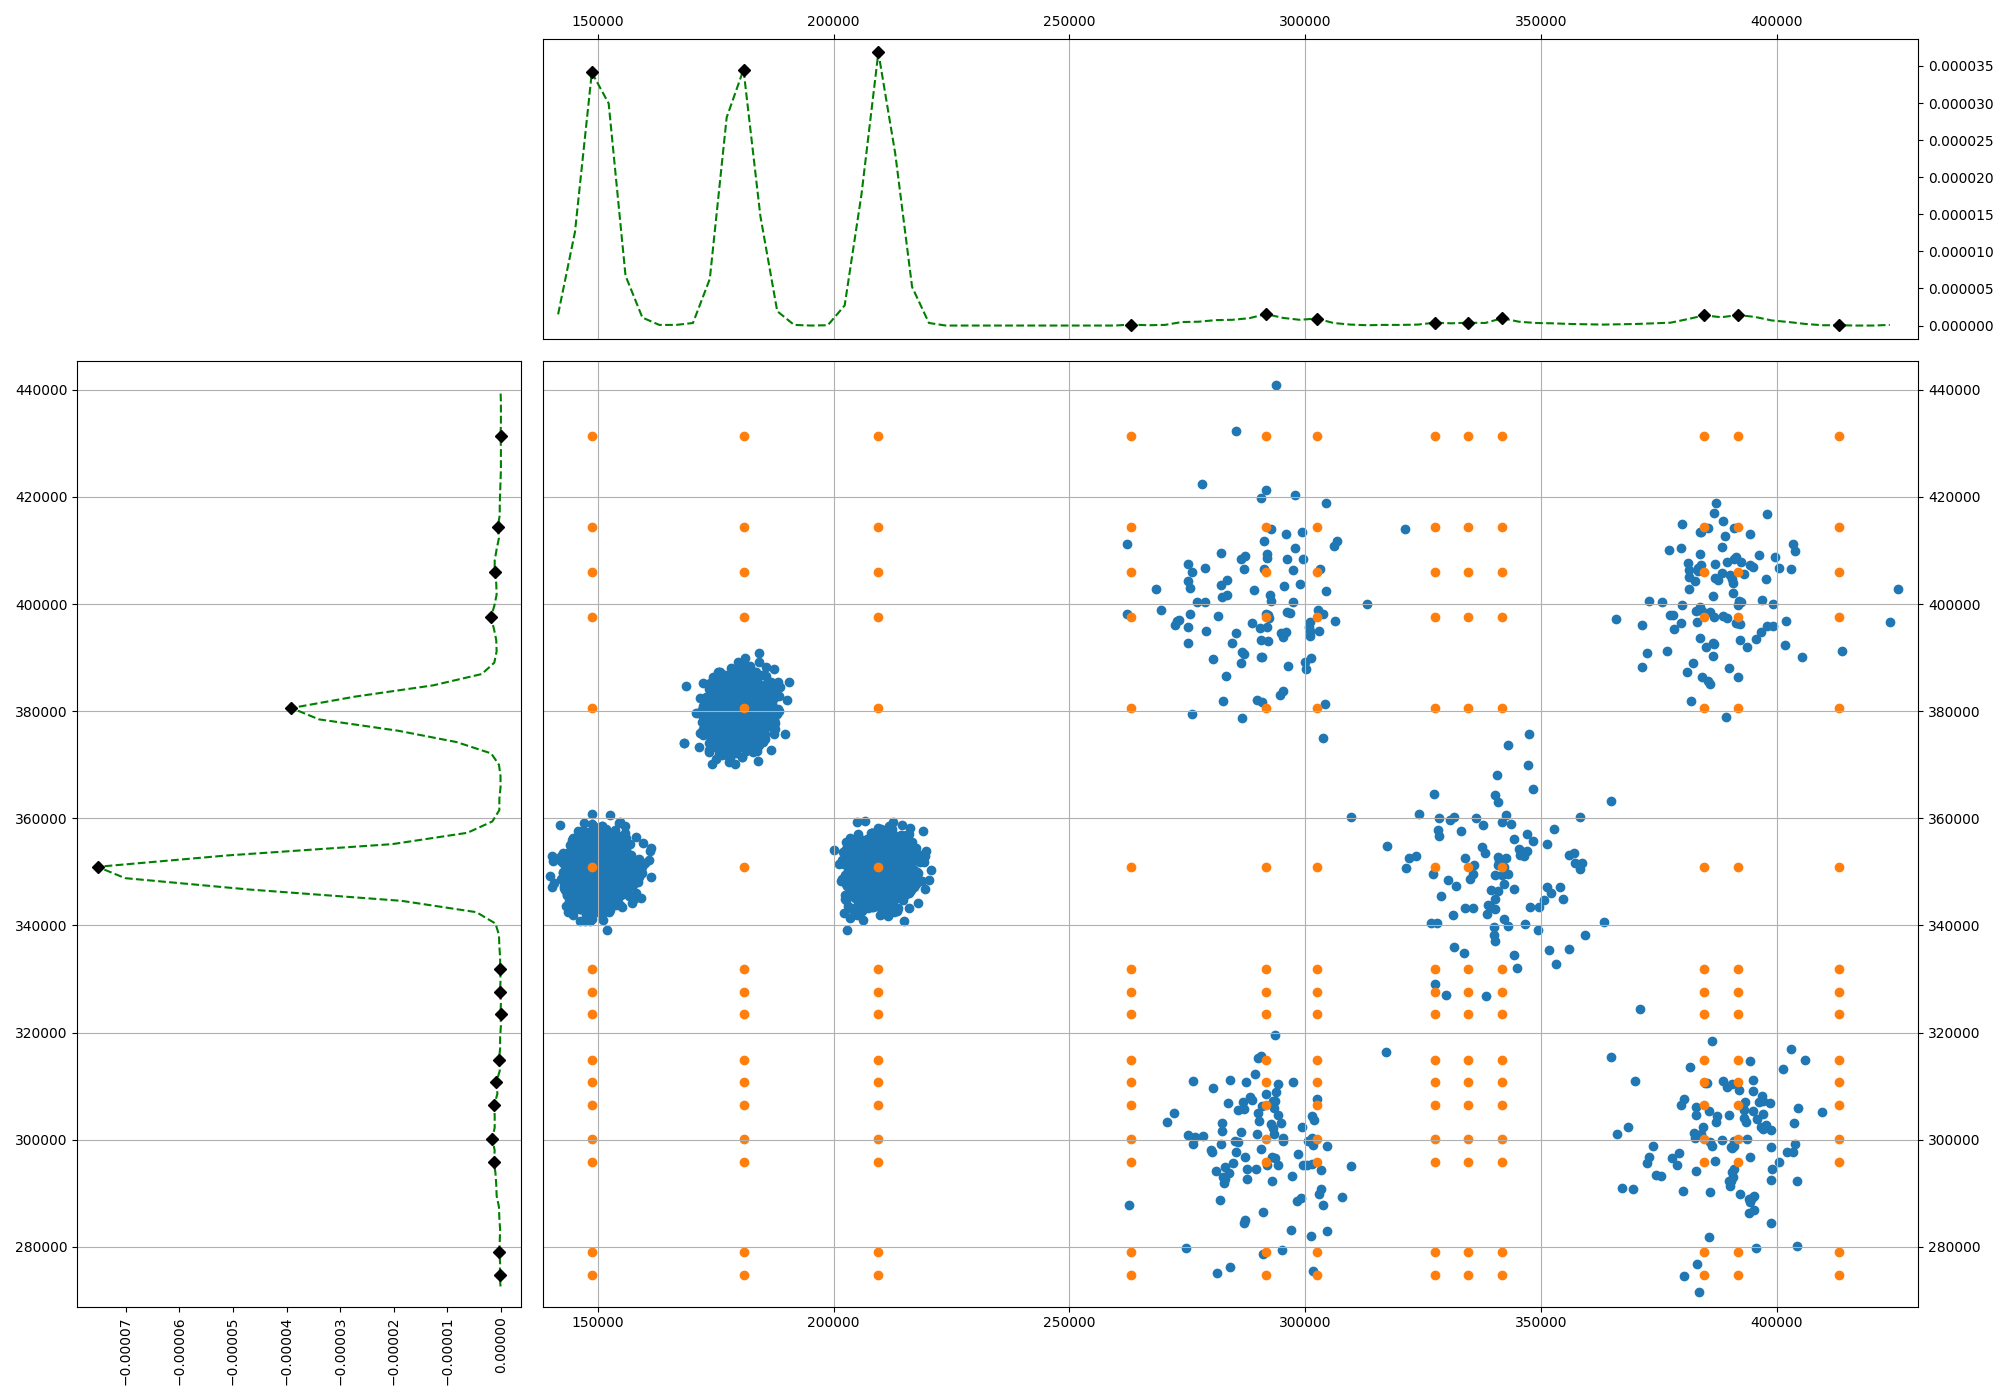
\includegraphics[width=0.7\textwidth]{unbalance_rescaled_coolfig.png}}
  \caption{The grid with all the potential centroids computed from the peaks.}
  \label{grid}
\end{figure*}

Moreover, among all the potential peaks created, only those which have at least one data
item assigned after a run of the k-means are kept. This allows to discard all the
false-positives that were found creating all the possible combinations in all the feature spaces.
Furthermore, it represents the refinement step for the algorithm.

Finally, the items in this grid are the initial centroids, representing both the value for the
$k$ parameter (i.e. the number of items in this grid) and their coordinates.


\subsection{Centroids refinement}
The other important phase is to find a good positioning of the $k$ initial centroids.
The main idea behind this feature is the following:
\begin{enumerate}
    \item \label{step1} use peaks' locations as the ones of the centroids.
    \item build an ellipse around every centroid with the $(a,b)$ parameters (namely the x-axis
        and the y-axis radii) applying the formula in Equation \ref{ellipse_params} (see
        Algorithm~\ref{alg:find_ellipses}).
    \item merge all the ellipses that intersect with each other (see
        Algorithm~\ref{alg:merge_procedure}).
    \item go to \ref{step1} until convergence or some other exit criterion is met.
\end{enumerate}

\begin{algorithm}[h]
    \KwIn{centroids, [(centroidId,x,y)]}
    \KwIn{clusters, [\{id: [(x, y)]\}]}
    \KwResult{ellipses}

    cDesnity = {}\;
    $dx$ = $dy$ = []\;
    \For{cluster $\in$ clusters}{
        $(x_{\mu}, x_{\sigma})$ = normFit (cluster.x)\;
        $(y_{\mu}, y_{\sigma})$ = normFit (cluster.y)\;

        $dx$ += px = normPDF $(x_{\mu}, x_{\mu}, x_{\sigma})$\;
        $dy$ += py = normPDF $(y_{\mu}, y_{\mu}, y_{\sigma})$\;

        cDensity[cluster.id] = $((x_{\mu}, x_{\sigma}, px), (y_{\mu}, y_{\sigma}, py))$\;
    }

    ellipses = []\;
    \For{$(c, ((x_x, x_y, x_p), (y_x, y_y, y_p))) \in$ cDensity}{
        ellipses += $(c$,\\
            $((x_x, x_y, (x_p - dx_{\mu})/dx_{\sigma})$, \\
            $(y_x, y_y,  (y_p - dy_{\mu})/dy_{\sigma})))$\;
    }

    \KwRet{ellipses}
    \caption{Compute Estimated Influence Area}\label{alg:find_ellipses}
\end{algorithm}

\begin{algorithm}[h]
    \KwIn{ellipses}
    \KwIn{cstats, \{id: (xsum, ysum, n)\}}
    \KwResult{centroids}

~\\
    // Fing merges
    merges = []
    \For{$e_0, e_1 \in ellipses$}{
        // Compute $a,b$ ellipse paramteres (Eq~\ref{ellipse_params})\\
        $eia_0$ = computeEIA ($e_0$)\;
        $eia_1$ = computeEIA ($e_1$)\;

        \If{$Ellipse(e_0, eia_0) \cap Ellipse(e_1, eia_1) \neq \varnothing$}{
            merges += $(e_0, e_1)$\;
        }
    }

~\\
    // Apply merges
    merged = {}\;
    \For{($e_0, e_1) \in merges$}{
        $e_0$ = findCurrentIdIfMerged ($e_0$, merged)\;
        $e_1$ = findCurrentIdIfMerged ($e_1$, merged)\;

        $(xsum_0, ysum_0, n_0)$ = cstats[$e_0$.id]\;
        $(xsum_1, ysum_1, n_1)$ = cstats[$e_1$.id]\;

        cstats[$e_0$.id] = \\
            $(xsum_0 + xsum_1, ysum_0 + ysum_1, n_0 + n_1)$\;
        merged[$e_1$.id] = $e_0$.id\;
    }

~\\
    // Derive centroids
    centroids = []\;
    \For{(c, (xsum, ysum, n)) $\in$ cstats}{
        centroids += $(xsum/n, ysum/n)$\;
    }

    \KwRet{centroids}
    \caption{Merge centroids with overlapping EIA}\label{alg:merge_procedure}
\end{algorithm}


The formula described in Equation~\ref{ellipse_params} computing the heigth and the width of
the ellipses is the key aspect of the proposed merging strategy.
\begin{equation}
\label{ellipse_params}
    f(\sigma, cdens) = ((\sigma * 2 * 0.35) + (cdens * 0.7)) * 5
\end{equation}
Where:
\begin{itemize}
    \item $\sigma$ is the standard deviation of the gaussian distribution underlying the cluster.
    \item $cdens$ is the value of the gaussian distribution Probability Distribution Function (PDF)
        in the mean.
\end{itemize}

To better understand the reasoning behind this formuls, a more precise explenation of its components
is needed.\\
Given the mean and the standard deviation of a cluster,
$\sigma$ is doubled to take both the sides of the gaussian distribution into account.
The 0.35 and the 0.7 values allow the density in the mean value of the gaussian distribution ($cdens$)
to influence more the size of the ellipse rather than its standard deviation ($\sigma$). Finally, 5 is
an overall scaling factor useful to allow the comparison of cluster with very different densities.

From an higher point of view, Equation \ref{ellipse_params} represents the \emph{Estimated Influence Area}
(EIA) for each cluster. As the name suggests, this depicts (also visually) the area of influence a
cluster has on all the others.\\
As it is possible to see from Figure~\ref{start}, the ellipses represent all the initial
\emph{EIAs} starting from all the potential centroids after discarding
all the centroids that has no item belonging to them (which are clearly false-positives).
If two clusters' estimated influence area has a non-empty intersection, it
means that they can be collapsed and become a single bigger cluster.
The Figures~\ref{start}, \ref{middle} and \ref{end} depicts the trend and the position of the
\emph{EIAs} during an example merging procedure.

Moreover, as it is possible to notice from Figure \ref{end}, the approach described in this
section started with many potential centroids (see Figure~\ref{start}) and after a
few iterations converged finding the 8 clusters in the dataset successfully
(see Figure~\ref{end}).

\begin{figure}[t]
  \center{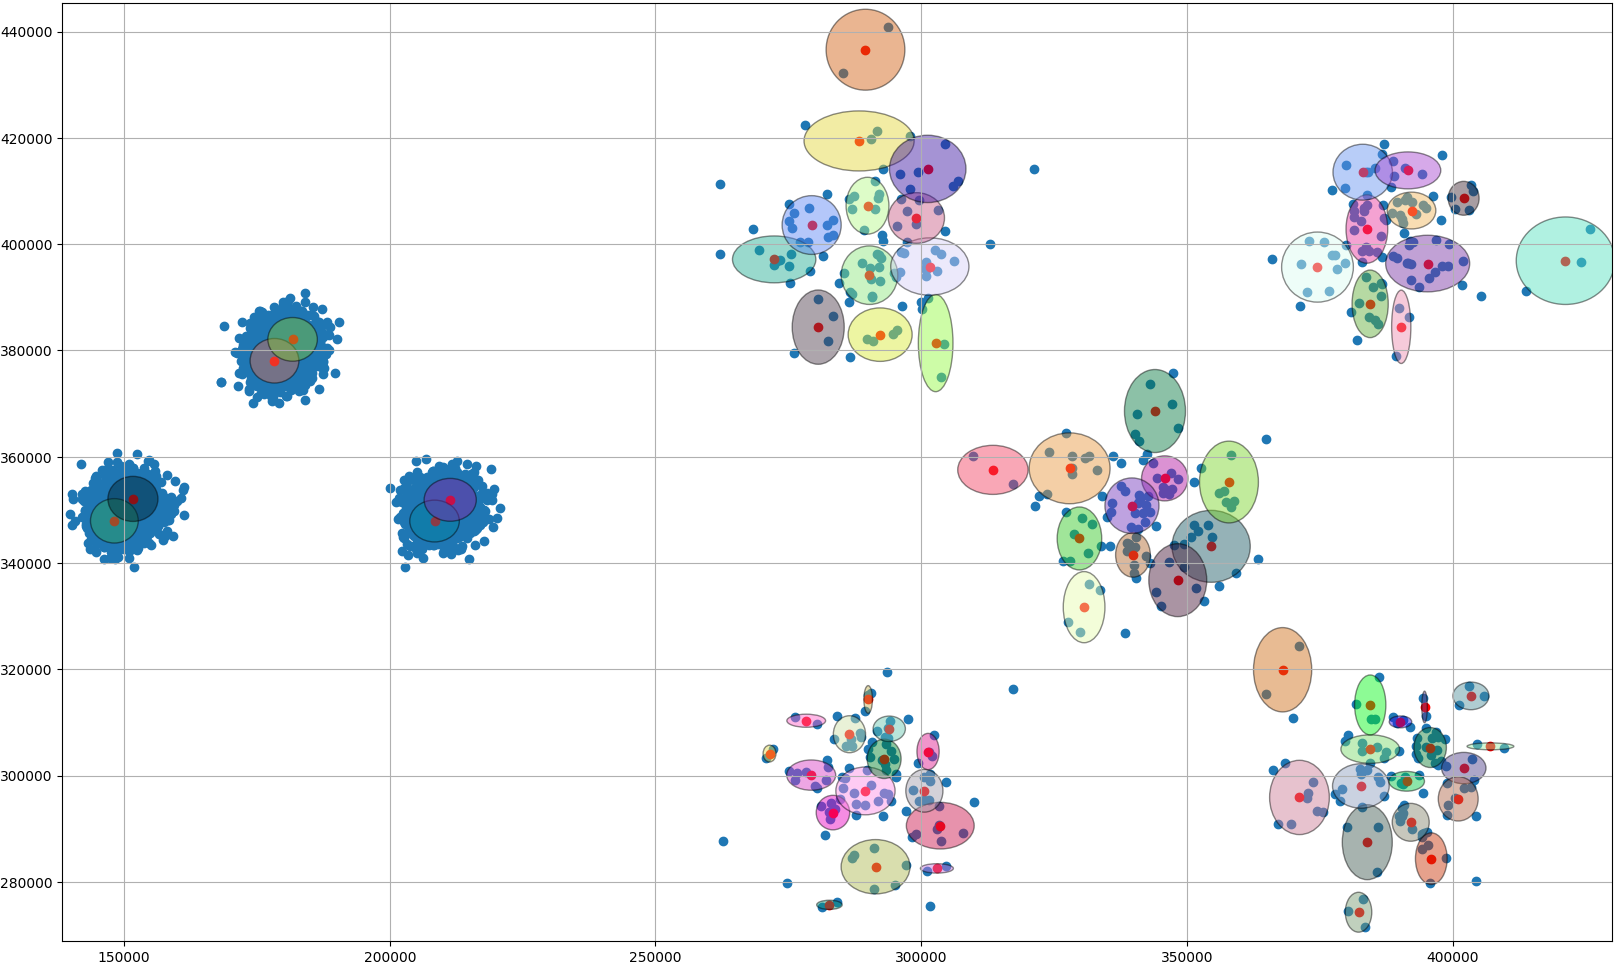
\includegraphics[width=0.5\textwidth]{unbalance_rescaled_density_0.png}}
  \caption{The first estimated influence areas after filtering some of the false-positives.}
  \label{start}
\end{figure}

\begin{figure}[t]
  \center{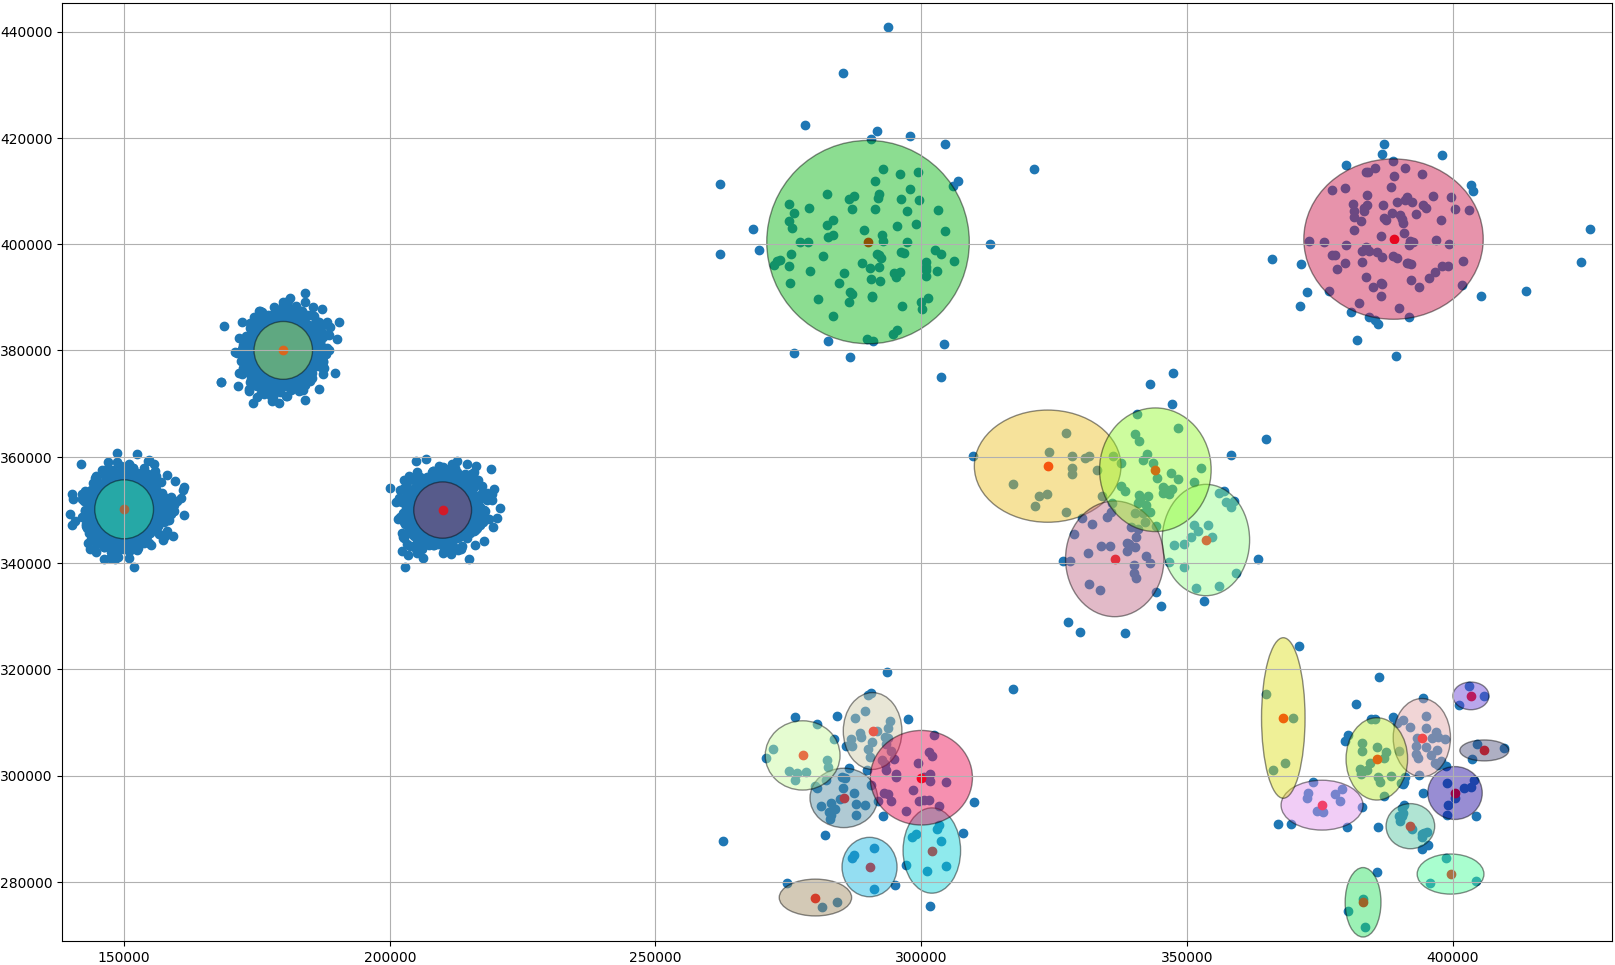
\includegraphics[width=0.5\textwidth]{unbalance_rescaled_density_3.png}}
  \caption{The situation after 4 iterations.}
  \label{middle}
\end{figure}

\begin{figure}[t]
  \center{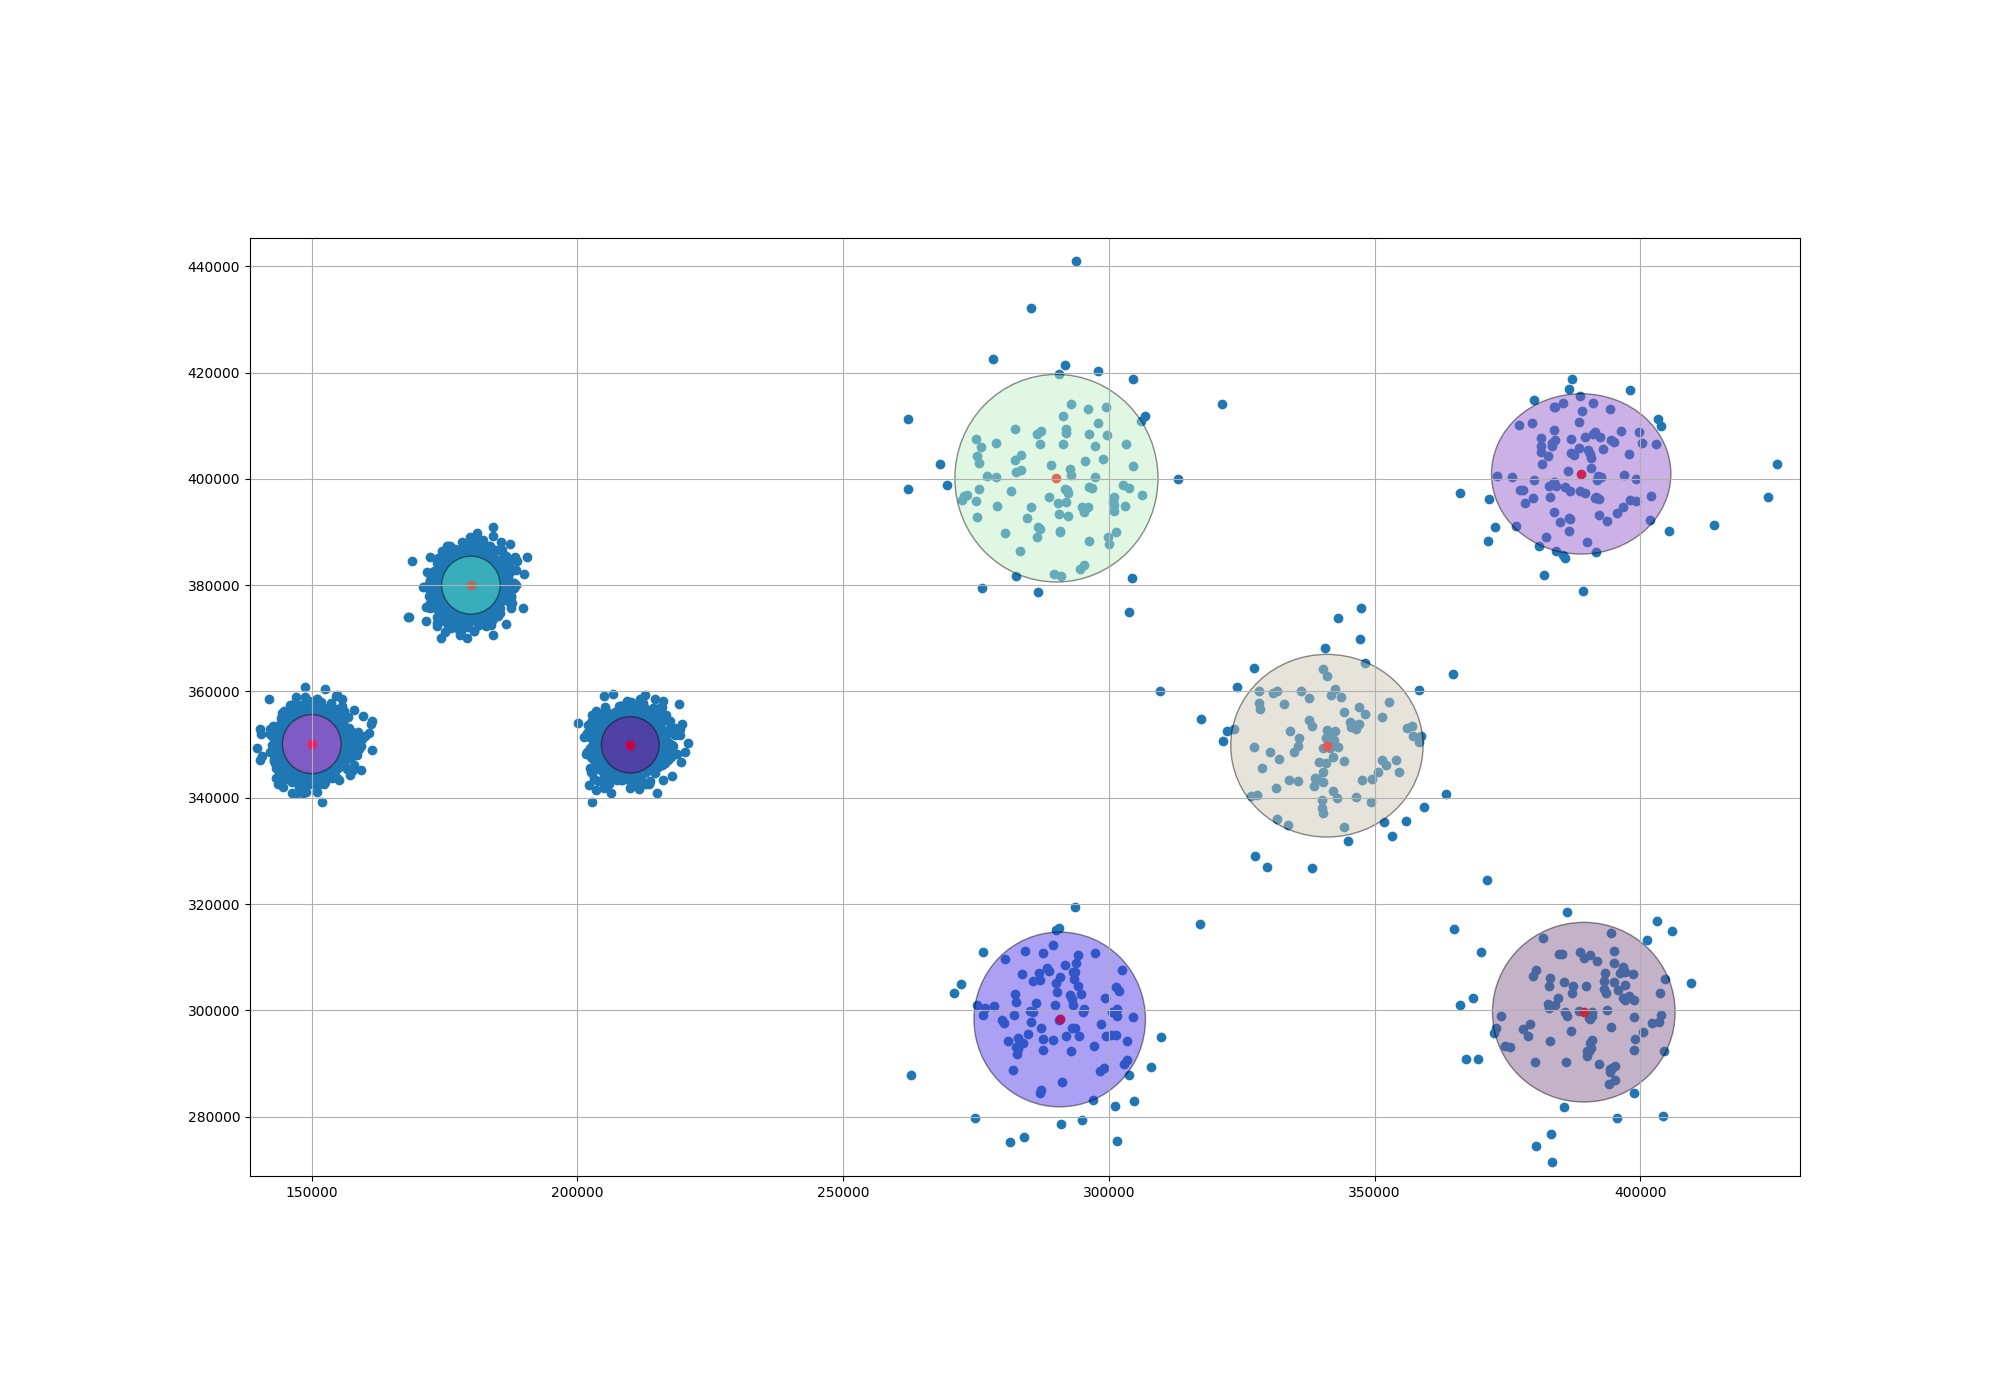
\includegraphics[width=0.5\textwidth]{unbalance_rescaled_density_6.png}}
  \caption{The final outcome of the algorithm.}
  \label{end}
\end{figure}

A noteworthy aspect is that all the aforementioned factors used inside Equation \ref{ellipse_params} have
been set after several tuning stages through empirical tests using many datasets with different
clusters' properties.

Nevertheless, representing the clusters by means of sufficient statistics allows to implement an $O(1)$
merging procedure. More in detail, every cluster is internally represented as a touple with the
following information:
\begin{equation*}
    \left(\left[\sum_{p}^{|C|} feat[0],\dots,\sum_{p}^{|C|} feat[n]\right],|C|\right)
\end{equation*}
In a 2-dimensional euclidean space, this metadata result in a list containing the the sum of all the
points' coordinates among the 2 axes and the number of points within the cluster taken into consideration.
This structure contains the least possible information to compute the centroid's coordinates as the
barycenter of that particolar cluster.

Finally, this merging strategy enables all the \emph{Data Mining Desiderata} mentioned in Section
\ref{intro}. It makes use of sufficient statistics to internally represent every cluster, hence
requiring an overall amount of memory that is linear in the number of peaks ($O(k)$, \emph{limited memory}
property). Furthermore, the \emph{online} behaviour is guaranteed by default, since the centroid
bootstrap and merging procedure always return a solution at any point in time. Finally, it allows
to deal with \emph{straming} data thanks both to its linear memory consumption and to its ability to
work with chunks of data by default, propagating all the sufficient statistics needed to update the
centroids from one iteration to another. This also guarantees that if the computation is stopped
it can be restarted without the need to re-process everything from scratch.


\subsection{Applications}
The approach presented in this work can have two main applications. On the one hand,
this procedure can be used as a bootstrapping phase for a  ``k-means''-like algorithm.
On the other, it can be integrated with other partitional clustering algorithms to
refine the local solution during the computation phase, allowing the system as a
whole to find increasingly better clusters.

Moreover, this work is agnostic with respect
to the metric used to compute the distance between the items. For the seek of
completeness, all the figures presented in this work are computed using a
standard euclidean distance.

\section{Valudation and experiments}
\label{experiments}
Several dataset~\cite{ClusteringDatasets} are used in order to evaluate the correctness 
of this solution. This phase is a very important in order to understand its potentialities.

The assessment is performed using input data that have very different properties,
starting from one with many small and dense cluster and ending with a dataset with few 
but very sparse clusters. In this way it is possible to see how the implementation
behaves under very different scenarios.

\begin{figure}[t]
  \center{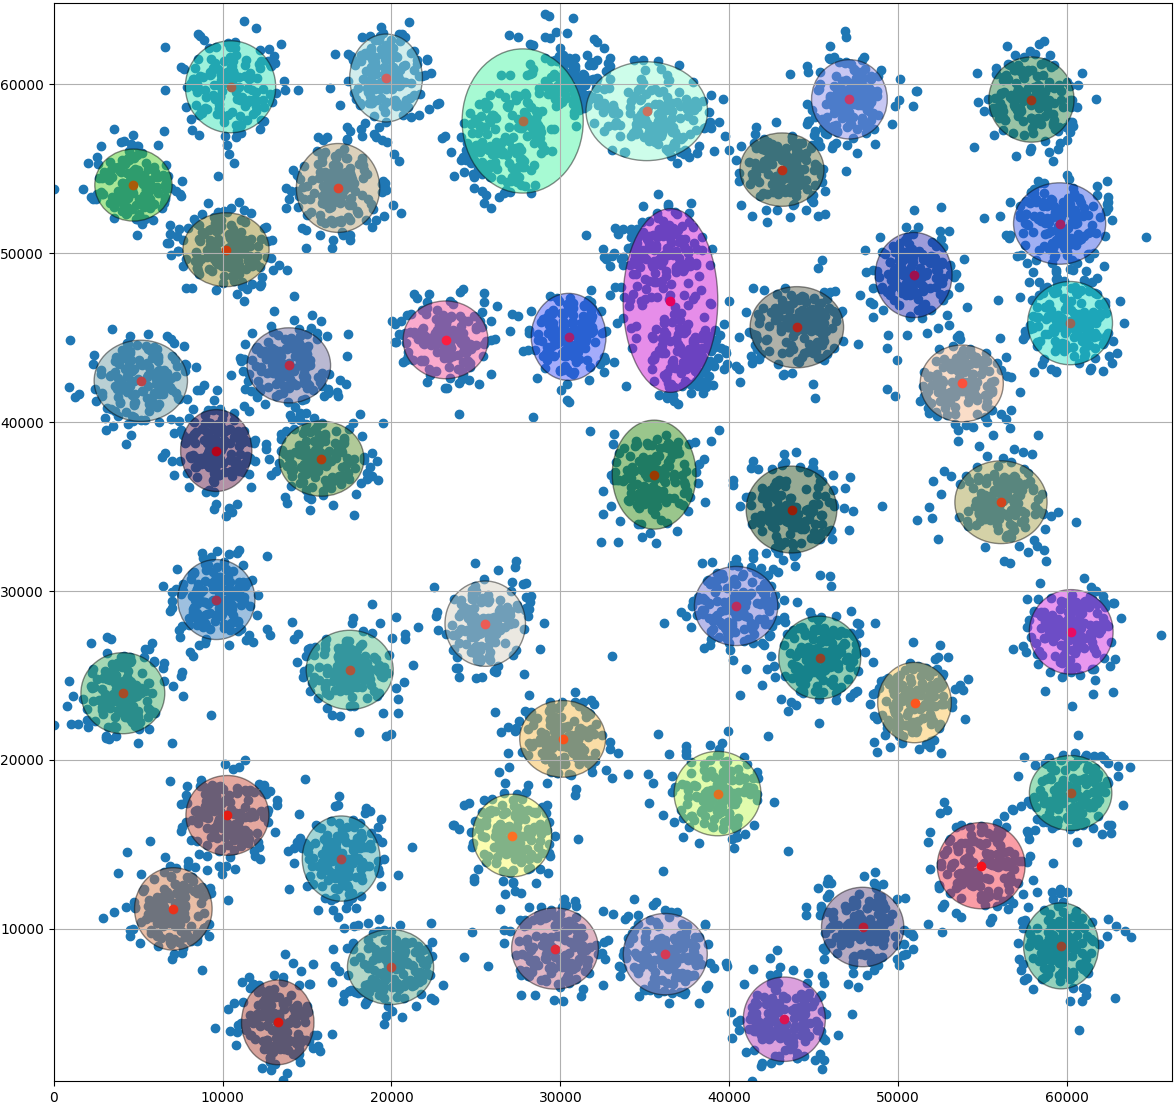
\includegraphics[width=0.5\textwidth]{a3_density_3.png}}
  \caption{The final outcome from a dataset with many small and dense regions.}
  \label{dataset1}
\end{figure}

\begin{figure}[t]
  \center{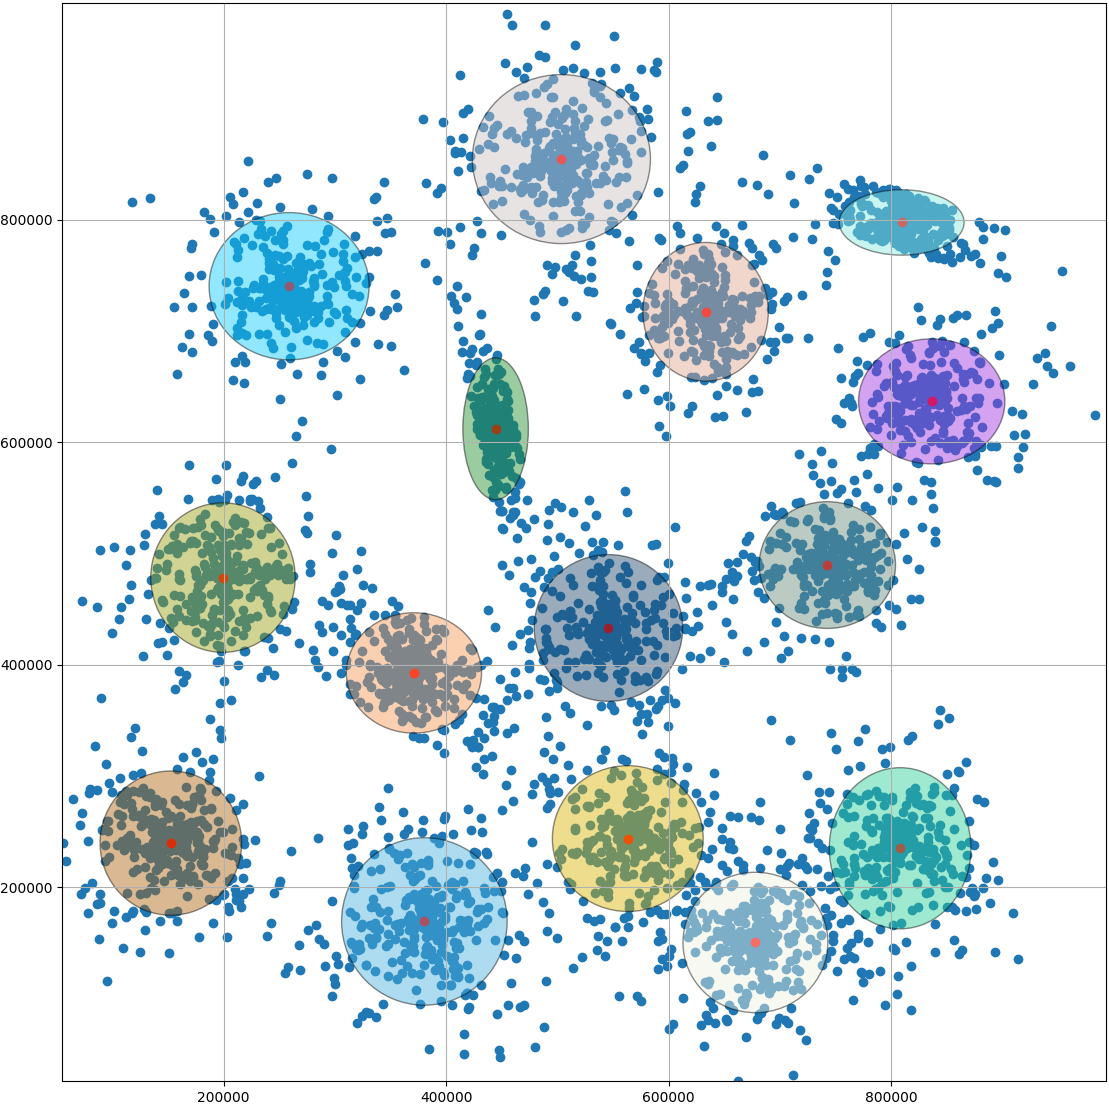
\includegraphics[width=0.5\textwidth]{s2_density_3.png}}
  \caption{The final outcome from a dataset with many small and quite sparse points.}
  \label{dataset2}
\end{figure}

\begin{figure}[t]
  \center{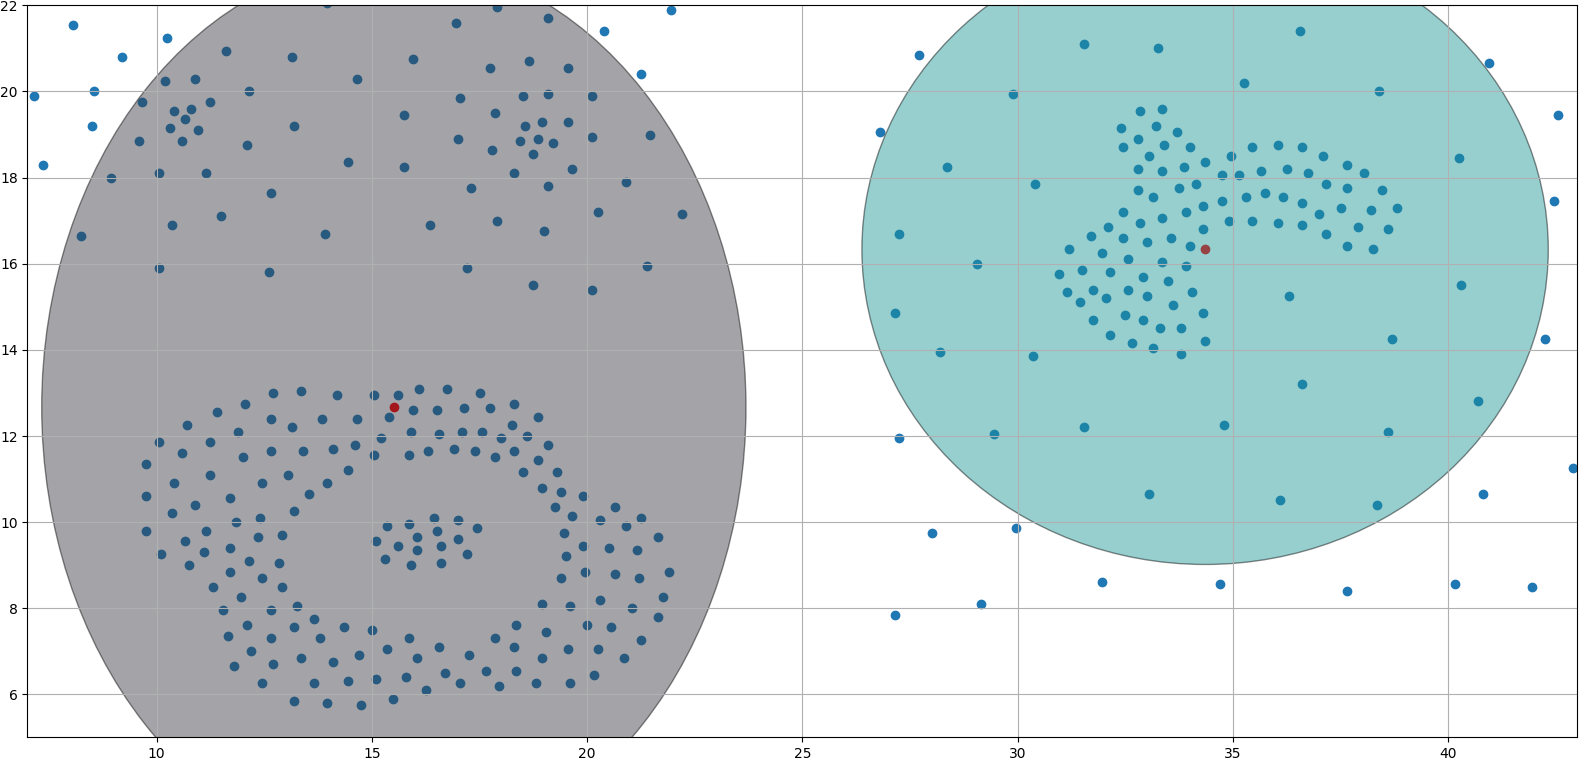
\includegraphics[width=0.5\textwidth]{Compound_density_1.png}}
  \caption{The final outcome from a very difficult dataset for a "k-means"-like algorithm.}
  \label{dataset3}
\end{figure}

As it is possible to see from Figure~\ref{dataset1} and \ref{dataset2}, this approach
succeeds both in finding the right number of clusters and in positioning the centroids, even
though the datasets cannot be considered "easy" ones for this kind of clustering
algorithms. 
Furthermore, Figure~\ref{dataset3} highlights how a dataset that visually can be 
divided into few different-shaped regions does not fit the capabilities of a partitioning
algorithm like the k-means. This is due to the distribution from which the points are
sampled, which are far from being a smooth bell-curved shape.
This particular example is clearly crafted to hinder the clustering algorithm under test.

\section{Conclusions and future work}
This work is a streaming, on-line and limited memory solution to the two most common
issues in the partitional clustering algorithms.
It has been tested against several datasets~\cite{ClusteringDatasets} with
very different characteristics in order to evaluate the overall performances that
can be achieved with this algorithm.
In addition, it provided promising results both in optimal and in several challenging
scenarios.

Moreover, a visual validation of the quality of the resulting clusters has
been performed in order to understand how this approach behaves under different
circumstances and to uncover its possible limitations.

Finally, this work discloses further optimizations that can be implemented to
improve the algorithm's performance both from the quantitative and the qualitative
points of view.


% remove eventually
% \cite{*}

%
% The following two commands are all you need in the
% initial runs of your .tex file to
% produce the bibliography for the citations in your paper.

\bibliographystyle{abbrv}
\bibliography{biblio}% biblio.bib is the name of the Bibliography in this case

% You must have a proper ".bib" file
%  and remember to run:
% latex bibtex latex latex
% to resolve all references
%
% ACM needs 'a single self-contained file'!
%

\end{document}
